\documentclass[
% -- opções da classe memoir --
12pt,				% tamanho da fonte
openright,			% capítulos começam em pág ímpar (insere página vazia caso preciso)
oneside,			% para impressão em recto e verso. Oposto a oneside
a4paper,			% tamanho do papel. 
% -- opções da classe abntex2 --
%chapter=TITLE,		% títulos de capítulos convertidos em letras maiúsculas
%section=TITLE,		% títulos de seções convertidos em letras maiúsculas
%subsection=TITLE,	% títulos de subseções convertidos em letras maiúsculas
%subsubsection=TITLE,% títulos de subsubseções convertidos em letras maiúsculas
% -- opções do pacote babel --
english,			% idioma adicional para hifenização
brazil				% o último idioma é o principal do documento
]{abntex2}

% ---
% Pacotes acrescentados
% ---
%\usepackage[portuguese, ruled, linesnumbered]{algorithm2e}
%\usepackage{algorithmic}

% ---
% Pacotes básicos 
% ---
\usepackage{lmodern}			% Usa a fonte Latin Modern			
\usepackage[T1]{fontenc}		% Selecao de codigos de fonte.
\usepackage[utf8]{inputenc}		% Codificacao do documento (conversão automática dos acentos)
\usepackage{lastpage}			% Usado pela Ficha catalográfica
\usepackage{indentfirst}		% Indenta o primeiro parágrafo de cada seção.
\usepackage{color}				% Controle das cores
\usepackage{url}				% Citar URLs
\usepackage{graphicx}			% Inclusão de gráficos
\usepackage{microtype} 			% para melhorias de justificação
\usepackage{booktabs}
\usepackage{multirow}
\usepackage[table]{xcolor}
\setlength{\aboverulesep}{0pt}
\setlength{\belowrulesep}{0pt}
\usepackage{scalefnt}
% ---

% ---
% Pacotes adicionais, usados apenas no âmbito do Modelo Canônico do abnteX2
% ---
\usepackage{lipsum}				% para geração de dummy text
\usepackage{amssymb}			% para uso de símbolos matemáticos
% ---

% ---
% Pacotes de citações
% ---
\usepackage[brazilian,hyperpageref]{backref}	 % Paginas com as citações na bibl
\usepackage[alf]{abntex2cite}	% Citações padrão ABNT

%VERONICA/ADIÇÃO/INICIO
%%%%%%%%%%%%%%%%%%%%%%%%%%%%%%%%%%%%%%%%%%
% Pacotes adicionais Wal/Veronica
%%%Para incluir um pdf
\usepackage[final]{pdfpages}
%\usepackage{lscape}
%\usepackage{pdflscape}

\usepackage{amsmath}

\usepackage{algorithm}
\usepackage{algpseudocode}
\usepackage{etoolbox}

%https://tex.stackexchange.com/questions/230497/change-name-of-algorithm
\makeatletter
\newenvironment{algoritmo}[1][htb]{%
	\renewcommand{\ALG@name}{Algoritmo}% Update algorithm name
	\begin{algorithm}[#1]%
	}{\end{algorithm}}
\makeatother

%https://tex.stackexchange.com/questions/292815/how-can-i-create-vertical-lines-indentation-in-algorithm-pseudo-code-correctly-w/292838
%%%%%%%%%%%%%%%%%%%%%%%%%%%%%%%%%%%%%%%%%%
\makeatletter
% start with some helper code
% This is the vertical rule that is inserted
\newcommand*{\algrule}[1][\algorithmicindent]{%
	\makebox[#1][l]{%
		\hspace*{.2em}% <------------- This is where the rule starts from
		\vrule height .75\baselineskip depth .25\baselineskip
	}
}

\newcount\ALG@printindent@tempcnta
\def\ALG@printindent{%
	\ifnum \theALG@nested>0% is there anything to print
	\ifx\ALG@text\ALG@x@notext% is this an end group without any text?
	% do nothing
	\else
	\unskip
	% draw a rule for each indent level
	\ALG@printindent@tempcnta=1
	\loop
	\algrule[\csname ALG@ind@\the\ALG@printindent@tempcnta\endcsname]%
	\advance \ALG@printindent@tempcnta 1
	\ifnum \ALG@printindent@tempcnta<\numexpr\theALG@nested+1\relax
	\repeat
	\fi
	\fi
}
% the following line injects our new indent handling code in place of the default spacing
\patchcmd{\ALG@doentity}{\noindent\hskip\ALG@tlm}{\ALG@printindent}{}{\errmessage{failed to patch}}
\patchcmd{\ALG@doentity}{\item[]\nointerlineskip}{}{}{} % no spurious vertical space
% end vertical rule patch for algorithmicx
\makeatother
%%%%%%%%%%%%%%%%%%%%%%%%%%%%%%%%%%%%%%%%%%

%https://github.com/filipesaraiva/algorithmic-portuguese
%http://linorg.usp.br/CTAN/macros/latex/contrib/algorithms/algorithms.pdf
%%
%% Copying and distribution of this file, with or without modification,
%% are permitted in any medium without royalty provided the copyright
%% notice and this notice are preserved.  This file is offered as-is,
%% without any warranty.
%%
%% Copyright (c) 2012-2015 Filipe de Oliveira Saraiva <mail@filipesaraiva.info>
%%

%% Entrada e sa�da do algoritmo

\renewcommand{\algorithmicrequire}{\textbf{Entrada:}}
\renewcommand{\algorithmicensure}{\textbf{Sa\'{i}da:}}

%% Vari�veis

%\renewcommand{\algorithmicinputs}{\textbf{entradas}}
%\renewcommand{\algorithmicoutputs}{\textbf{sa\'{i}das}}
%\renewcommand{\algorithmicglobals}{\textbf{globais}}
\renewcommand{\algorithmicreturn}{\textbf{retorna}}

%% Miscel�nea: inicializadores e terminadores de blocos, comandos diversos

\renewcommand{\algorithmicdo}{\textbf{fa\c{c}a}}
%\renewcommand{\algorithmicto}{\textbf{at\'{e}}}
\renewcommand{\algorithmicend}{\textbf{fim}}
%\renewcommand{\algorithmicprint}{\textbf{imprime}}

%% Estruturas booleanas

%\renewcommand{\algorithmictrue}{\textbf{verdadeiro}}
%\renewcommand{\algorithmicfalse}{\textbf{falso}}

%% Estruturas e conectores l�gicos

%\renewcommand{\algorithmicand}{\textbf{e}}
%\renewcommand{\algorithmicor}{\textbf{ou}}
%\renewcommand{\algorithmicxor}{\textbf{xou}}
%\renewcommand{\algorithmicnot}{\textbf{n\~{a}o}}

%% Estruturas condicionais

\renewcommand{\algorithmicif}{\textbf{se}}
\renewcommand{\algorithmicthen}{\textbf{ent\~{a}o}}
\renewcommand{\algorithmicelse}{\textbf{sen\~{a}o}}
%\renewcommand{\algorithmicelsif}{\algorithmicelse\ \algorithmicif}
%\renewcommand{\algorithmicendif}{\algorithmicend\ \algorithmicif}

%% Estruturas de repeti��o

\renewcommand{\algorithmicwhile}{\textbf{enquanto}}
%\renewcommand{\algorithmicendwhile}{\algorithmicend\ \algorithmicwhile}

\renewcommand{\algorithmicfor}{\textbf{para}}
\renewcommand{\algorithmicforall}{\textbf{para todo}}
%\renewcommand{\algorithmicendfor}{\algorithmicend\ \algorithmicfor}

\renewcommand{\algorithmicloop}{\textbf{loop}}
%\renewcommand{\algorithmicendloop}{\algorithmicend\ \algorithmicloop}

\renewcommand{\algorithmicrepeat}{\textbf{repita}}
\renewcommand{\algorithmicuntil}{\textbf{at\'{e}}}

%%%%%%%%%%%%%%%%%%%%%%%%%%%%%%%%%%%%%%%%%%
%VERONICA/ADIÇÃO/FIM

% Pacotes adicionais Wal
\usepackage{subfig}  %para exibir figuras lado a lado
\usepackage{listings} % Para inclusao de codigos fontes
\usepackage{color}
\definecolor{mygreen}{rgb}{0,0.6,0}
\definecolor{mygray}{rgb}{0.5,0.5,0.5}
\definecolor{mymauve}{rgb}{0.58,0,0.82}
\lstset{ %
	backgroundcolor=\color{white},   % choose the background color; you must add \usepackage{color} or \usepackage{xcolor}
	basicstyle=\footnotesize,        % the size of the fonts that are used for the code
	breakatwhitespace=false,         % sets if automatic breaks should only happen at whitespace
	breaklines=true,                 % sets automatic line breaking
	captionpos=t,                    % sets the caption-position to bottom
	commentstyle=\color{mygreen},    % comment style
	deletekeywords={...},            % if you want to delete keywords from the given language
	escapeinside={\%*}{*)},          % if you want to add LaTeX within your code
	extendedchars=true,              % lets you use non-ASCII characters; for 8-bits encodings only, does not work with UTF-8
	frame=single,	                 % adds a frame around the code
	keepspaces=true,                 % keeps spaces in text, useful for keeping indentation of code (possibly needs columns=flexible)
	keywordstyle=\color{blue},       % keyword style
	language=Octave,                 % the language of the code
	otherkeywords={*,...},           % if you want to add more keywords to the set
	numbers=left,                    % where to put the line-numbers; possible values are (none, left, right)
	numbersep=5pt,                   % how far the line-numbers are from the code
	numberstyle=\tiny\color{mygray}, % the style that is used for the line-numbers
	rulecolor=\color{black},         % if not set, the frame-color may be changed on line-breaks within not-black text (e.g. comments (green here))
	showspaces=false,                % show spaces everywhere adding particular underscores; it overrides 'showstringspaces'
	showstringspaces=false,          % underline spaces within strings only
	showtabs=false,                  % show tabs within strings adding particular underscores
	stepnumber=1,                    % the step between two line-numbers. If it's 1, each line will be numbered
	stringstyle=\color{mymauve},     % string literal style
	tabsize=2,	                   	 % sets default tabsize to 2 spaces
	title=\lstname,                  % show the filename of files included with \lstinputlisting; also try caption instead of title
	numberbychapter=false
}


% --- 
% CONFIGURAÇÕES DE PACOTES
% --- 

\hyphenation{a-di-cio-nal-men-te}

% ---
% Configurações do pacote backref
% Usado sem a opção hyperpageref de backref
\renewcommand{\backrefpagesname}{Citado na(s) página(s):~}
% Texto padrão antes do número das páginas
\renewcommand{\backref}{}
% Define os textos da citação
\renewcommand*{\backrefalt}[4]{
	\ifcase #1 %
	Nenhuma citação no texto.%
	\or
	Citado na página #2.%
	\else
	Citado #1 vezes nas páginas #2.%
	\fi}%
% ---

%-----
%Adaptações do formato ABNT para UNESP
\addto\captionsbrazil{
	\renewcommand{\listfigurename}{Lista de Figuras}
	\renewcommand{\listtablename}{Lista de Tabelas}
	\renewcommand{\listadesiglasname}{Lista de Abreviaturas e Siglas}
	%\renewcommand{\folhadeaprovacaoname}{Folha de Aprovação}
	\renewcommand{\listadesimbolosname}{Lista de Símbolos}
}
%-----

%Comandos para padronização - Wal
\newcommand{\suporte}{\textit{suporte}}
\newcommand{\confianca}{\textit{confiança}}
\newcommand{\itemset}{\textit{itemset}}
\newcommand{\itemsets}{\textit{itemsets}}
\newcommand{\kitemset}{\textit{k-itemset}}
\newcommand{\kitemsets}{\textit{k-itemsets}}
\newcommand{\nitemset}[1]{\textit{#1-itemset}}
\newcommand{\nitemsets}[1]{\textit{#1-itemsets}}
\newcommand{\apriori}{\textit{Apriori}}
\newcommand{\cl}{\textit{Clustering}}
\newcommand{\sky}{\textit{Sky}}
%\newcommand{\ABNTEXfontereduzidaTiny}{\tiny}
%\newcommand{\ABNTEXfontereduzidaScriptsize}{\scriptsize}
%\newcommand{\ABNTEXfontereduzidaSmall}{\small}


% ---
% Informações de dados para CAPA e FOLHA DE ROSTO
% ---
\uppercase{\titulo{SISTEMA DE MANUTENÇÂO DE MENSALIDADES DE ACADEMIA COM DIVERSAS MODALIDADES}}
\autor{GABRIEL LUIZ}
\local{Rio Claro - SP}
\data{2019}
\orientador[Orientadora:]{Profa. Dra. Simone das Graças Domingues Prado}
\instituicao{%
	UNIVERSIDADE ESTADUAL PAULISTA
	\par
	``J\'ULIO DE MESQUITA FILHO''
	\par
	Instituto de Geociências e Ciências Exatas - IGCE
	\par
	Curso de Bacharelado em Ciências da Computação}

\tipotrabalho{Trabalho de Graduação}
% O preambulo deve conter o tipo do trabalho, o objetivo, 
% o nome da instituição e a área de concentração 
\preambulo{Relatório de Linguagens Comerciais de Programação, realizado de janeiro à julho de 2019, visando desenvolver uma plataforma java pelo Curso de Bacharelado em Ciências da Computação do Instituto de Geociências e Ciências Exatas da Universidade Estadual Paulista “Júlio de Mesquita Filho”, Câmpus de Rio Claro. }
% ---

% ---
% Configurações de aparência do PDF final

% alterando o aspecto da cor azul
\definecolor{blue}{RGB}{41,5,195}

% informações do PDF
\makeatletter
\hypersetup{
	%pagebackref=true,
	pdftitle={\@title}, 
	pdfauthor={\@author},
	pdfsubject={\imprimirpreambulo},
	pdfcreator={regras de associação},
	pdfkeywords={mineração de dados}{inciacao cientifica}{unesp}, 
	colorlinks=false,       		% false: boxed links; true: colored links
	linkcolor=blue,          	% color of internal links
	citecolor=blue,        		% color of links to bibliography
	filecolor=magenta,      		% color of file links
	urlcolor=blue,
	bookmarksdepth=4
}
\makeatother
% --- 

% --- 
% Espaçamentos entre linhas e parágrafos 
% --- 

% O tamanho do parágrafo é dado por:
\setlength{\parindent}{1.3cm}

% Controle do espaçamento entre um parágrafo e outro:
\setlength{\parskip}{0.2cm}  % tente também \onelineskip

% ---
% compila o indice
% ---
\makeindex
% ---

% ----
% Início do documento
% ----
\begin{document}
	
	% Seleciona o idioma do documento (conforme pacotes do babel)
	%\selectlanguage{english}
	\selectlanguage{brazil}
	
	% Retira espaço extra obsoleto entre as frases.
	\frenchspacing 
	
	% ----------------------------------------------------------
	% ELEMENTOS PRÉ-TEXTUAIS
	% ----------------------------------------------------------
	
	\pretextual
	
 	  \begin{capa}
	\begin{center}
	\Large\imprimirinstituicao
	\end{center}

	\begin{center}
	\vspace*{3.4cm}
	\Large GABRIEL LUIZ
	\linebreak
	\Large LEO EDUARDO
	\linebreak
	\Large GUILHERME SIMIONATTO
	\vspace*{1.5cm}
	
	\Large \textbf{\imprimirtitulo}
	
	\vspace*{2.4cm}
	
	\noindent Orientadora: Profa. Dra. Simone das Graças Domingues Prado
	
	\vspace*{2.4cm}
	
	{\large\imprimirlocal}
	\par
	{\large\imprimirdata}
	\vspace*{1cm}
	\end{center}
  \end{capa}
	
	\begin{folhaderosto}
	\begin{center}		
		
		\vspace*{\fill}\vspace*{\fill}
		\begin{center}
			\ABNTEXchapterfont\bfseries\Large\imprimirtitulo
		\end{center}
		\vspace*{\fill}
		
		\hspace{.45\textwidth}
		\begin{minipage}{.5\textwidth}
			\SingleSpacing
			\imprimirpreambulo
		\end{minipage}%		
		
		\vspace*{1cm}
		\begin{flushright}
			\noindent Alunos:  Gabriel Luiz
			\linebreak
			\noindent Guilherme Simionato
			\linebreak
			\noindent Leo Eduardo
		\end{flushright}
		\vspace*{1cm}
		\begin{flushright}
			\noindent Orientadora: Profa. Dra. Simone das Graças Domingues Prado
		\end{flushright}
		\vspace*{1cm}
				
				
		{\large\imprimirlocal}
		\par
		{\large\imprimirdata}
		\vspace*{1cm}
		
	\end{center}
\end{folhaderosto}
	
	%\include{errata}
	
	%\include{folhadeaprovacao}
	
	%\include{dedicatoria}
	
	%\include{agradecimentos}
	
	%\include{epigrafe}
	
	%\setlength{\absparsep}{18pt} % ajusta o espaçamento dos parágrafos do resumo
	%\include{resumo}
	
	
%\pdfbookmark[0]{\listfigurename}{lof}
%\listoffigures*
%\cleardoublepage
% ---

% ---
% inserir lista de tabelas
% ---
%\pdfbookmark[0]{\listtablename}{lot}
%\listoftables*
%\cleardoublepage
% ---

% ---
% inserir lista de algoritmos
% ---
%\pdfbookmark[0]{Lista de Algoritmos}{loa}
%\listofalgorithms
%\cleardoublepage
% ---

% ---
% Lista de scripts
% ---
%\pdfbookmark[0]{Lista de Scripts}{loa}
%\lstlistoflistings
%\cleardoublepage

% ---
% inserir lista de abreviaturas e siglas
% ---
%\begin{siglas}
%	\item[KDD] Knowledge Discovery in Databases
%	\item[MD] Mineração da Dados
%	\item[MO] Medida Objetiva
%	\item[RA] Regra de Associação
%\end{siglas}
% ---

%\newpage
%\listofalgorithms*       % Lista de algoritmos
%\addcontentsline{toc}{section}{Lista de Algoritmos}

% ---
% inserir o sumario
% ---
\pdfbookmark[0]{\contentsname}{toc}
\tableofcontents*
\cleardoublepage
% ---

	
	% ----------------------------------------------------------
	% ELEMENTOS TEXTUAIS
	% ----------------------------------------------------------
	\textual
	
	%Capitulos
	\chapter{Introdução}\label{cap_intro}

Este relatório visa exibir o processo de desenvolvimento realizado durante o primeiro semestre do ano de dois mil e dezenove, referente a um sistema de academia, prentendedo-se efetuar o cadastro de diversos alunos e diversas modalidades, com descontos quando ocorrer a execução de mais de uma modalidade, se ofertado.

Dados os objetivos, este trabalho encontra-se estruturado da seguinte maneira: o Capítulo 2 aborda o processo de desenvolvimento do software. Por fim, no Capítulo~\ref{cap_conclu} são dadas as considerações finais a respeito deste relatório de linguagens comerciais de programação...

	\chapter{Desenvolvimento}\label{cap_intro}
A proposta deste projeto se baseia no desenvolvimento de uma aplicação para controle de mensalidades oferecidas por uma academia para seus alunos, onde os pagamentos mensais podem, de acordo com os pacotes escolhidos pelos alunos, sofrer descontos.

Estes descontos devem ser concedidos aos alunos que escolherem um pacote que contempla mais de uma modalidade. Por exemplo:

\begin{figure}[H]
	\centering
	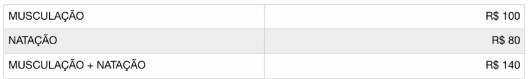
\includegraphics[width=0.7\linewidth]{images/exModalidades}
	\caption{Exemplo de modalidades}
	Fonte: pessoal.
	\label{fig:exModalidades}
\end{figure}

Para a execução deste sistema, no escopo inicial foi proposto três telas, porém no atual projeto contemplaremos apenas duas, sendo elas cadastro e consulta. Na tela de cadastro será possível realizar todos os cadastros do sistema da academia (Alunos, Modalidades e valores, vinculos Aluno x Modalidade/Pacote, etc), enquanto na tela de consulta podemos visualizar a situação das mensalidades dos alunos (Pendente/Vencidas/Pagas) e aplicar filtros de pesquisa.

Na tela de cadastro será informado, no módulo de aluno, informações mínimas como: documento, endereço, nome, modalidade/pacote etc. Já no módulo de modalidades faremos o cadastro dos tipos de modalidades oferecidas (a princípio apenas o nome) e seus respectivos valores, bem como os pacotes ofertados. Sendo assim, a construção das tabelas se dá conforme segue:

\begin{figure}[H]
	\centering
	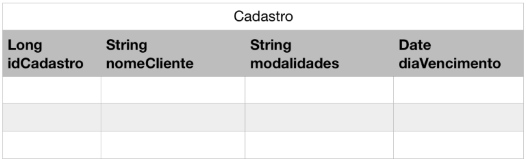
\includegraphics[width=0.7\linewidth]{images/tabelaCadastro}
	\caption{Tabela cadastro}
	Fonte: pessoal.
	\label{fig:tabelaCadastro}
\end{figure}

\begin{figure}[H]
	\centering
	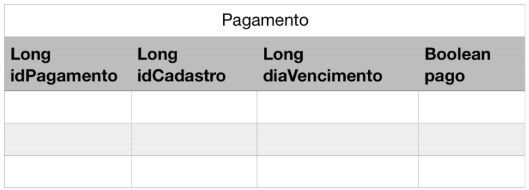
\includegraphics[width=0.7\linewidth]{images/tabelaPagamento}
	\caption{Tabela Pagamento}
	Fonte: pessoal.
	\label{fig:tabelaPagamento}
\end{figure}

Usaremos as tecnologias de Java e Swing (para o código e telas), MongoDB (para estruturar o banco de dados), Spring (para comunicação com o banco de dados) e GIT (para o gerenciamento de versão) para criar este sistema que pretende facilitar a consulta de pagamentos pendentes e controlar a matrícula dos alunos. Além disso, o atual escopo não prevê um controle financeiro (retorno de troco, quantidade recebida ou ainda fechamento de contas a pagar) e pode, futuramente, ser melhorado com a implementação destes itens ou ainda relatórios, controle de usuário etc.
	\chapter{Tecnologias}\label{cap_tecnologias}

\section{Tecnologias}
Neste trabalho foram usadas diversas tecnologias para auxiliar no processo de desenvolvimento, onde este projeto que poderia ser utilizado também para ser projetado telas web onde o backend foi desenvolvido para aceitar requisições web e salvar ou realizar pesquisas. 

\subsection{Java 8 e Mavan}
Dentre estas tecnologias a linguagem Java na versão 8 (ou superior) conforme utilizada em sala de aula, maven como ferramenta de automação de compilação "O Maven utiliza um arquivo XML (POM) para descrever o projeto de software sendo construído, suas dependências sobre módulos e componentes externos."\cite{maven}. 

\subsection{Spring e Lombok}
É utilizado do spring para realizar a conexão com o banco de dados e expor os endpoints utilizados na aplicação, juntamente com o lombok que é utilizado para facilitar o desenvolvimento evitando ter que digitar todos os getters e setters e disponibilizando um builder para facilitar a maneira de instanciar um objeto.

\subsection{MongoDB e ORM}
Foi utilizado o banco de dados não relacional mongodb com ORM (Object Related Model), "ORM ou Object Relational Mapping é uma técnica de mapeamento objeto relacional que visa criar uma camada de mapeamento entre nosso modelo de objetos (aplicação) e nosso modelo relacional (banco de dados) de forma a abstrair o acesso ao mesmo."\cite{orm} onde as classes em java se tornam tabelas no banco de dados e é possível realizar consultas através da classe que extende o banco de dados.

\subsection{IDE Intellij}
Também foi utilizado da IDE intellij para facilitar o desenvolvimento "O IDE e um programa de computador, geralmente utilizado para aumentar a produtividade
dos desenvolvedores de software, bem como a qualidade desses produtos. Podem auxiliar,
através de ferramentas e características, na redução de erros e na aplicação de técnicas
como o RAD (Rapid Application Development)" \cite{ide}

\subsection{GitHub}
Também foi feito o uso da ferramenta de controle de versão GitHub para gerenciar os arquivos de desenvolvimento e também deste relatório


	\chapter{Conhecimentos Utilizados aprendidos na disciplina}\label{ch-aula}

\section{Conhecimentos}

A disciplina de Linguagens Comerciais de Programação abordou diversos conceitos da linguaguem java. Dentre eles conexão cliente e servidor, coleções, classes, tipos, swing para desenvolvimento das telas, threads, banco de dados, 

	\chapter{Conclusão}\label{cap_conclu}

Conforme exposto na seção anterior, utilizou-se dos conhecimentos lecionados pela professora Simone das Graças Domingues Prado durante o primeiro semetre de dois mil e dezenove para realização da aplicação que visa permitir a consulta de pagamentos pendentes e controle de matrícula dos alunos de uma academia. Além disso, para o desenvolvimento foi necessário o conhecimento e aprendizado de outras tecnologias não abordadas em aula, mas que complementam o conteúdo como Spring, MongoDB e GIT.

Os realizadores deste projeto acreditam ter aplicado os conhecimentos passados em aula e realizado um projeto pertinente ao proposto.

Também foi possíveis perceber que é totalmente viável um desenvolvimento de um software que possa atender a todos os tipos de academias.


	
	
	% ----------------------------------------------------------
	% Finaliza a parte no bookmark do PDF
	% para que se inicie o bookmark na raiz
	% e adiciona espaço de parte no Sumário
	% ----------------------------------------------------------
	\phantompart
	
	%\chapter{Conclusão}
	
	
	% ----------------------------------------------------------
	% ELEMENTOS PÓS-TEXTUAIS
	% ----------------------------------------------------------
	\postextual
	% ----------------------------------------------------------
	
	% ----------------------------------------------------------
	% Referências bibliográficas
	% ----------------------------------------------------------
	\bibliography{references}
	
\end{document}
